\subsection{冻结策略下的全部原始记录生产}
全量实际尝试并形成终态 11,386 条、1,173,410 点，处理失败 0 条。所有分区都包含在生产中；这些汇总描述本数据集输出，不是新的独立最终测试。发布策略为 S0，运行不需要逐记录模型或在线记忆，未加入逐记录候选拒绝后回退机制。原坐标、时间和记录身份保持可追踪。

\begin{table}[H]\centering\small
\caption{全部原始记录的生产终态。分母包含开发、选择、确认和其余记录；同一输入的参考与发布策略分别处理。}
\begin{tabularx}{\linewidth}{@{}Yrr@{}}\toprule 读数 & R0 & S0 \\ \midrule
原始记录 & 11,386 & 11,386 \\
原始点 & 1,173,410 & 1,173,410 \\
S 过滤点 & 501,511 & 1,199 \\
D 删除点 & 36,056 & 39,732 \\
P 精简点 & 435,373 & 911,330 \\
显式保留点 & 200,470 & 221,149 \\
共同覆盖原始点 & 671,899 & 1,172,211 \\
覆盖原始窗口 & 15,205 & 24,764 \\
无输出记录 & 4,859 & 0 \\
跨原始断点边 & 0 & 0 \\
\bottomrule\end{tabularx}\end{table}

全部点以互斥终态记账，共同覆盖另算。发布策略的最大 P 即时误差为 4.999964 工作米；共同 raw-to-final 最大误差为 368.707060 工作米，两者参考集合不同。未因合法空输出而删去原始记录，也未将参考空记录记作处理异常。

\subsection{新增覆盖的边界案例：不能解释为新增干净点}
逐记录保护在全部 11,386 条上满足，6,522 条严格改善，共同覆盖增加 500,312 个原始身份。这个读数只说明固定定义下的覆盖恢复；全量新增覆盖最大偏差为 266.016754 工作米，明显大于确认样本中的新增覆盖最大值。

按 R0 的真实过滤原因，将新增覆盖互斥分解为：仅长度不足 492,513 点、仅点数不足 5,434 点、同时满足两项 2,365 点。这三项之和才是全部新增覆盖；不能把它们统一解释为长度小于 65。新增覆盖身份最终有 20,679 点被显式保留、475,957 点由 P 精简、3,676 点由 D 删除。后两类仍可能被最终折线的相邻保留索引夹持，所以共同覆盖增长远大于存储点增长。

实际最差点位于记录 352 的原始索引 105。完整局部原始窗口为 [104, 105, 106, 107]，共 4 点；R0 因点数不足过滤该段，原因是 \texttt{TOO\_FEW\_POINTS}，并非长度小于 65。S0 保留该段后，D 以方向规则删除索引 105，P 的完整输入与输出同为 [104, 106, 107]，这个局部没有 P 删除。该原始点到最终夹持边 [104, 106] 的偏差由独立 Decimal 原值重算确认；整条记录的 P 即时最大误差仍只有 4.344986 工作米。

因此，新增覆盖不意味着新增点已被识别为干净，DP 自身的 5 工作米保证也没有覆盖此前被 D 删除的点。参考短段过滤条件是“点数不足或长度不足”的并集；开发中的观察不能替代全量过滤原因。本案例保留为发布局限，没有在看过全量之后更换策略或修改保护定义。

\subsection{扩大范围的工作坐标核验与限制}
全部 1,173,410 点和 11,386 条记录完成指定 ENU 与独立 PROJ 路径核对，最大实现差为 \texttt{8.1481e-10} 工作米。原始相邻边 1,162,024 条全部核查；与同假设椭球测地距离的最大绝对差 0.452041 工作米，最大相对差 0.015054\%。

实际处理的 S 邻边 2,324,048、段长 51,926、D 窗口 1,844,110 与 P 完整输入点 1,768,322 均进入登记的阈值/误差/保留集合敏感性核验。登记的替代模型阶段检查未观察到动作差异。没有进行全域所有点的两两距离；公式核对和模型近似比较不能证明源 datum。

独立 C 对完整原始范围、身份、阶段操作、点账本和汇总逐记录核验；另外从预登记随机组与所有实际存在类别中抽取数学复算记录。随机部分 40 条，加上每个类别至多两个完整组代表后共 50 条、100 份策略轨迹接受独立 Decimal/PROJ 重算。这是明确的数学抽查，不是所有同类记录都用第二套数学实现重跑。

替代坐标的独立阶段敏感性复算覆盖 56 条、112 份策略轨迹，包含预登记随机/类别代表、全部已报告差异及极值记录。它在真实各阶段固定输入上比较动作；没有把这种检查写成另一坐标模型下的全链重跑，也没有声称全部未抽中记录的敏感性均被独立重算。

\begin{figure}[H]\centering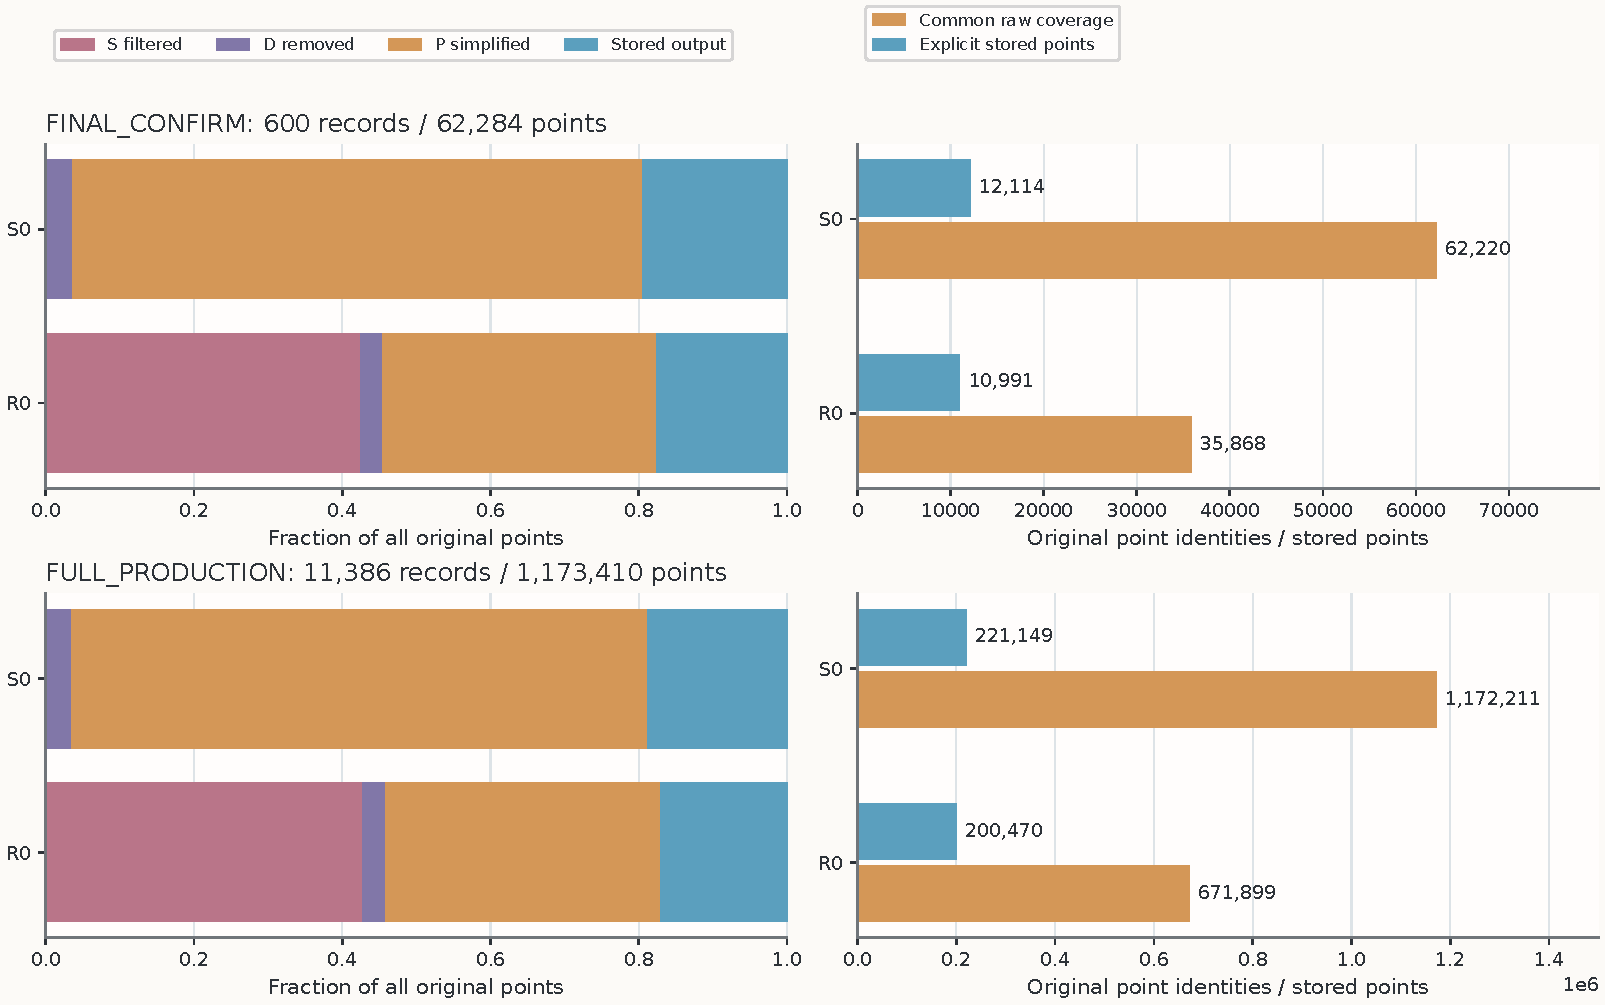
\includegraphics[width=.98\linewidth]{../../figures/goal3/point_fates_and_coverage.pdf}
\caption{最终确认与全量生产的互斥点终态、共同覆盖和显式存储点，分别使用各自完整分母。}\end{figure}
\begin{figure}[H]\centering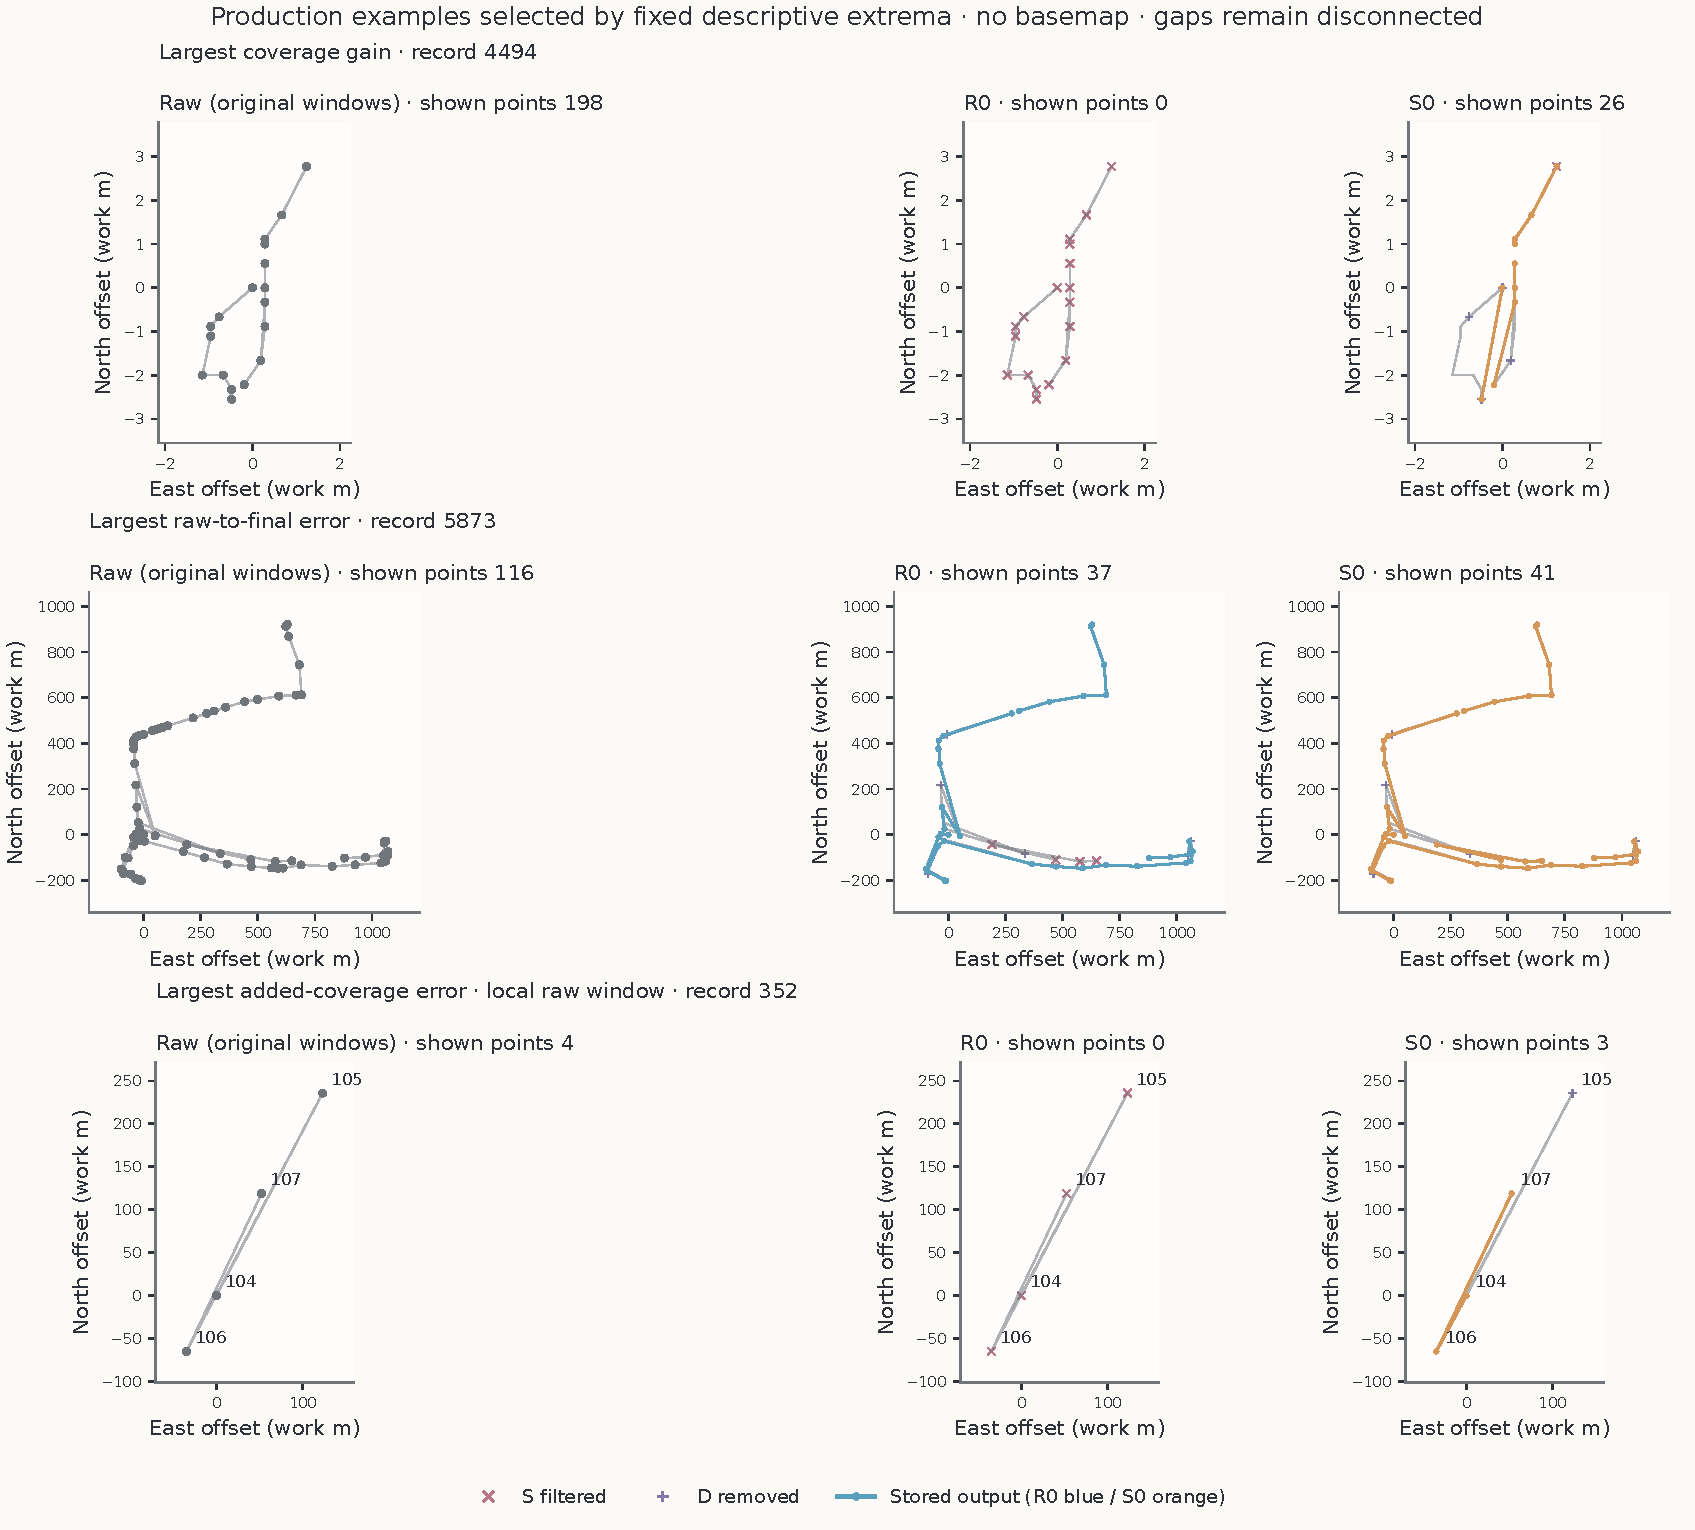
\includegraphics[width=.98\linewidth]{../../figures/goal3/production_trajectory_cases.pdf}
\caption{同案例的原始、R0 与发布策略。前两行分别选取最大覆盖增益和最大原始几何误差的完整记录；第三行为新增覆盖最差点所在的四点局部窗口，图中显示点数不是整条记录的存储总数。粉红叉号表示 S 过滤，紫色加号表示 D 删除；蓝色与橙色折线分别表示 R0 与 S0 的存储输出。同一行原点与尺度一致，断段不重连，无道路底图。}\end{figure}
\subsection{执行成本与复现身份}
\begin{table}[H]\centering\small
\caption{当前有效运行的计算账本。观察数可以复用相同配置或已经存在的真实产物，不等于实际重新处理次数。}
\begin{tabularx}{\linewidth}{@{}Yrrrr@{\hspace{1.4em}}r@{}}\toprule 运行范围 & 实际处理 & 缓存复核 & 同配置复用 & 策略观察 & 秒 \\ \midrule
最终开发对照 & 600 & 1,680 & 360 & 2,640 & 130.6 \\
选择 & 708 & 0 & 252 & 960 & 61.3 \\
最终确认 & 1,200 & 0 & 0 & 1,200 & 93.7 \\
全量生产 & 22,772 & 0 & 0 & 22,772 & 1763.6 \\
\bottomrule\end{tabularx}\end{table}

表中只列当前四个有效运行，不把早期开发、失效后重建、独立核验或 Notebook 离线复算的成本塞入同一分母。各次耗时包含其实际执行环境，不作为硬件无关基准。四次运行新增记录级模型调用均为 0；原生治理角色的工具事件另记，底层请求与费用未知。历史真实提议在默认离线复算中原样重用，不能计作新的 LIVE 提议。
